% Paper for CCGrid 2027, Track 5 (Performance Modeling, Analysis, and Optimization).
% Limit: 10 IEEE pages including references; double-blind review (no names, no repository links).
% Build: make (latexmk -pdf). \todo{} marks what is still missing.
\documentclass[conference]{IEEEtran}
\usepackage[utf8]{inputenc}
\usepackage[T1]{fontenc}
\usepackage{cite}
\usepackage{amsmath,amssymb}
\usepackage{graphicx}
\usepackage{booktabs}
\usepackage{array}
\usepackage{xcolor}
\usepackage{url}
\usepackage[hidelinks]{hyperref}
% anonymous PDF: no creation/modification dates (time zone) and no creator strings
\pdfinfoomitdate=1
\pdftrailerid{}
\hypersetup{pdfcreator={},pdfproducer={},pdfauthor={},pdftitle={}}
\usepackage{cleveref}
% For the final submission: switch to \usepackage[disable]{todonotes}
\usepackage[disable]{todonotes}
\newcommand{\anonrepo}{\url{https://anonymous.4open.science/r/mesh-overhead-artifact-7FD0/}}
\graphicspath{{figs/}}

\begin{document}

\title{Sidecars, Ambient, or eBPF? Measuring the Tail-Latency and Resource Cost of Kubernetes Service Meshes}

% Double-blind: no names, affiliations, or e-mails
\author{\IEEEauthorblockN{Anonymous Author(s)}
\IEEEauthorblockA{Anonymous Institution}}

\maketitle

\begin{abstract}
Service meshes add encryption, telemetry, and traffic policy to microservices, but each data-plane design pays for
them differently: a proxy per pod (sidecar), a per-node L4 proxy with optional shared L7 waypoints (ambient), or
in-kernel eBPF with a per-node proxy. We measure seven configurations---no mesh, Istio sidecar, Istio ambient with and
without waypoints, Linkerd, and Cilium with WireGuard, with and without L7 policy---each in its default data path,
on a pinned, virtualized Kubernetes testbed with open-loop load at three fixed rates per application, using a
synthetic echo service, Online Boutique, and DeathStarBench Hotel Reservation. On Online Boutique at the middle
rate, the Istio sidecar adds 52\,ms to p99 latency and ambient L4 6.7\,ms, and the meshes keep 2.0 (Cilium without
L7) to 9.1 (Cilium with L7) more cores busy per 1{,}000~req/s than no mesh; energy per request grows by 16 to
188\% at the highest rate. Among meshes that authenticate workloads, ambient L4 has the lowest latency,
CPU, and memory and the highest or near-highest throughput; Cilium without L7 policy uses less CPU and sustains more throughput, with
lower or similar p99 except on the echo benchmark, but authenticates only nodes.
Profiling attributes most of the overhead
to HTTP/2 processing for the Istio sidecar, TLS for ambient L4, and, for Cilium, the redirect to its per-node
Envoy and Hubble flow logging, not its eBPF programs (4--5\% of its data-plane CPU). A compositional model
predicts the held-out application's p99 overhead within 11--13\% for the two L4 data planes, and a bottleneck law
predicts saturation throughput within 19\% on the two microservice applications; but neither per-hop costs, cross-node hops, nor node utilization
predict the tail of L7 data planes; the load on the busiest proxy instance predicts it better for per-pod sidecars,
and relieving the busiest node changed the sidecar's tail by only 4\%. We distill the
results into a decision guide for choosing a data plane.
\end{abstract}

\begin{IEEEkeywords}
service mesh, Kubernetes, tail latency, performance evaluation, eBPF, energy efficiency
\end{IEEEkeywords}

% ---------------------------------------------------------------------------------------------------------------
% 01-introduction.tex
\section{Introduction}
\label{sec:intro}

Service meshes have become the default way to add mutual TLS, fine-grained
traffic policy, and request-level telemetry to microservices on Kubernetes,
without changing application code. The price is paid on every request: traffic
that used to flow directly between two pods now crosses one or more proxies,
each of which terminates connections, encrypts and decrypts traffic, and often
parses application-layer protocols. In deep call graphs, this cost is paid at
every hop, and it shows up where operators care most: in the tail of the
latency distribution and in the CPU that must be provisioned for it.

The design space of service meshes has changed considerably in the last few
years. The original \emph{sidecar} architecture, in which a proxy runs next to
every application container (Istio with Envoy, Linkerd with its Rust
\texttt{linkerd2-proxy}), now competes with \emph{sidecar-less} designs. Istio
Ambient splits the data plane into a per-node L4 proxy (ztunnel) and optional,
shared L7 proxies (waypoints), while Cilium implements L3/L4 functions in eBPF
inside the kernel and delegates L7 processing to a per-node Envoy. Each design
moves work to a different place (the pod, the node, or the kernel) and changes
how many proxies a request traverses, so their costs cannot be inferred from
one another.

The most detailed study of mesh overheads to date, MeshInsight~\cite{zhu2023meshinsight},
decomposed the cost of the Istio sidecar into its components and found that it
can raise latency by up to 269\% and CPU usage by up to 163\%. That analysis,
however, covers only the Envoy sidecar, profiles it with at most one
outstanding request, and its model explicitly cannot predict tail latency. More recent comparisons of sidecar and
sidecar-less meshes~\cite{bremlerbarr2024mtls} examine mTLS alone, on a
synthetic server with an artificial delay, without L7 processing, waypoints,
energy, or a predictive model. Operators choosing a mesh today therefore lack a
same-testbed comparison of the architectures they can actually deploy.

This paper provides that comparison. We measure seven configurations on the same
testbed: no mesh, Istio sidecar, Istio Ambient with and without a waypoint,
Linkerd, and Cilium service mesh with and without L7 policy, each with east-west encryption enabled
in its default data path: workload-level mutual TLS for Istio and Linkerd,
and node-to-node WireGuard for Cilium. We drive an echo
microbenchmark and two widely used microservice benchmarks, Online
Boutique~\cite{onlineboutique} and Hotel Reservation from
DeathStarBench~\cite{gan2019deathstarbench}, with open-loop load, which avoids
the coordinated-omission bias that hides tail
latency~\cite{tene2015latency,schroeder2006open}.
Our contributions are:

\begin{itemize}
  \item \textbf{A same-testbed measurement of seven mesh configurations}
        (RQ1). We report p99 and p99.9 latency, maximum SLO-compliant
        throughput, CPU, memory, and energy per request, with ten randomized
        repetitions per cell for latency and resources (five for Cilium
        without L7 policy), three for energy, and
        non-parametric statistics. Sidecar-based
        Istio sustains only 30\% of the no-mesh throughput on the echo
        benchmark, while ambient L4 mode retains 78\%.
  \item \textbf{An attribution of overhead beyond Envoy} (RQ2). Using perf and
        eBPF, we break the cost down into TLS, L7 parsing, socket I/O, context
        switches, and kernel time, including ztunnel, the Ambient waypoint,
        \texttt{linkerd2-proxy}, and Cilium's agent, per-node Envoy, and
        WireGuard. Ablations show that Cilium's cost comes from the L7
        redirect and Hubble flow logging, not from its eBPF programs.
  \item \textbf{A model of the tail and its limits} (RQ3). A compositional
        model of per-hop proxy cost, cross-node hops, and queueing, fitted on
        two applications, explains the p99 of the third within 11--13\% for
        the L4 data planes; for per-pod sidecars, queueing at the busiest
        proxy instance cuts the error from 82\% to 19\% (Linkerd) and from
        135\% to 52\% (Istio), while node utilization does not explain it.
        Node utilization bounds throughput within 19\% on the two
        microservice applications. A placement experiment shows that node
        load explains the tail of L7 data planes only partly.
  \item \textbf{A decision guide} (RQ4) that maps latency, CPU, and energy
        budgets to the mesh that satisfies them.
\end{itemize}

We also partially reproduce MeshInsight: the CPU overhead of the Istio
sidecar on Online Boutique falls within the published range, but its latency
overhead is larger (\cref{sec:validation}). We release the testbed, scripts, and data to
support reproduction at \anonrepo.

The rest of the paper is organized as follows. \Cref{sec:background} describes
the mesh architectures we compare, \cref{sec:related} discusses related work,
\cref{sec:method} presents the testbed and methodology, and
\cref{sec:rq1,sec:rq2,sec:rq3,sec:rq4} answer the four research questions.
\Cref{sec:threats} discusses threats to validity and \cref{sec:conclusion}
concludes.

% 02-background.tex -- draft.
\section{Background: Service Mesh Data Planes}
\label{sec:background}

A service mesh has a \emph{control plane}, which distributes identities,
certificates, and routing policy, and a \emph{data plane}, which handles
application traffic. Our measurements concern the data plane, whose
architecture determines how many proxies a request crosses and where their work
is executed. \Cref{tab:configs} summarizes the configurations we study.

\paragraph{Per-pod sidecars}
In Istio's sidecar mode, an Envoy proxy is injected into every pod, and
iptables rules redirect all inbound and outbound traffic through it. A request
between two services therefore traverses two proxies, each of which terminates
TCP, performs mTLS, and parses HTTP or gRPC to apply L7 policy and collect
telemetry. Linkerd uses the same pattern with \texttt{linkerd2-proxy}, a
purpose-built proxy written in Rust that implements a smaller feature set.

\paragraph{Istio Ambient}
Ambient mode removes the sidecar. A per-node proxy, ztunnel, captures pod
traffic and carries it between nodes over mTLS in an HTTP CONNECT-based tunnel
(HBONE). ztunnel provides L4 functions only: identity, encryption, and L4
authorization. When L7 features are required, traffic is additionally routed
through a \emph{waypoint}, a shared Envoy deployment that serves a namespace or
a service account. Ambient therefore has two operating points, L4-only (IA4)
and L4 plus waypoint (IA7), which we measure separately.

\paragraph{Cilium service mesh}
Cilium implements networking, load balancing, and L3/L4 policy with eBPF
programs attached to the kernel datapath. Transparent encryption between nodes
uses WireGuard (or IPsec), and L7 policy is enforced by redirecting the matching
traffic to an Envoy instance shared by all pods on the node. Unlike the other
meshes, Cilium encrypts at the node level rather than per workload, and only
traffic subject to an L7 rule is sent through a proxy.

\paragraph{Where the cost goes}
These designs differ in three ways that matter for performance: the number of
user-space proxies on the request path (two for sidecars, zero to two for
Ambient and Cilium), whether those proxies are dedicated to a pod or shared by
a node, and how much work is moved into the kernel. Shared proxies amortize
memory but concentrate CPU on the node that hosts them, which, as we show in
\cref{sec:rq1}, matters for tail latency under load.

\begin{table}[t]
  \centering
  \caption{Configurations measured. All meshes run with mutual authentication
           and encryption enabled.}
  \label{tab:configs}
  \footnotesize
  \setlength{\tabcolsep}{4pt}
  \begin{tabular}{@{}lll@{}}
    \toprule
    ID  & Configuration            & Data plane on the path \\
    \midrule
    B   & No mesh (Cilium CNI)     & none \\
    IS  & Istio sidecar            & Envoy in every pod \\
    IA4 & Istio Ambient, L4        & per-node ztunnel \\
    IA7 & Istio Ambient + waypoint & ztunnel + per-namespace Envoy \\
    LK  & Linkerd                  & \texttt{linkerd2-proxy} in every pod \\
    CI  & Cilium service mesh      & eBPF, WireGuard, per-node Envoy \\
    \bottomrule
  \end{tabular}
\end{table}

% 03-related.tex -- draft. Re-read Meshlib and Cvetkovic & Klimovic before submission.
\section{Related Work}
\label{sec:related}

\paragraph{Component-level analysis of sidecars}
MeshInsight~\cite{zhu2023meshinsight} is the work closest in method to ours.
It profiles the Istio sidecar (Istio 1.13, Envoy 1.21) on Online Boutique and
Hotel Reservation and attributes its overhead to seven components, finding that
protocol parsing dominates. It reports latency increases of 27--269\% and CPU
increases of 42--163\%, depending on configuration, and proposes a linear
compositional model of overhead. The authors note that the model does not
predict tail latency, and that extending the analysis to other meshes is future
work. We extend the analysis to ztunnel, the Ambient waypoint,
\texttt{linkerd2-proxy}, and Cilium's eBPF datapath, use open-loop load, add
energy, and model the tail through a queueing term.

\paragraph{Comparisons of sidecar and sidecar-less meshes}
Bremler-Barr et al.~\cite{bremlerbarr2024mtls} compare Istio sidecar, Istio
Ambient (ztunnel only), Linkerd, and Cilium, focusing on the cost of mTLS. Their
workload is a synthetic server with a fixed 200\,ms delay driven by Fortio, and
they do not exercise L7 processing, waypoints, or realistic call graphs. They
also observe that Cilium does not encrypt traffic between pods on the same node,
a caveat that applies to our setup as well: under our placement, 2.8 of the
3.8 internal calls per Hotel Reservation request, and 0.6 of the 11 per Online
Boutique request, stay on one node and are therefore not encrypted by Cilium's
WireGuard. Our study uses multi-service
applications, includes the waypoint, and reports energy and a predictive model.

\paragraph{Reducing mesh overhead}
A separate line of work proposes new data-plane designs rather than measuring
existing ones. Meshlib~\cite{mostafaei2026meshlib} enforces mesh policy inside
the application process for sidecar-less meshes, and Cvetkovi\'c and
Klimovic~\cite{cvetkovic2025lightweight} design a lightweight sidecar-based mesh
for serverless platforms, where Ambient is not compatible with the platform.
\todo{re-read both papers and summarize their measured baselines in one
sentence each} Our measurements are complementary: they quantify the cost these
designs aim to remove, on the architectures in production today.

\paragraph{Microservice benchmarks and load generation}
We use Online Boutique~\cite{onlineboutique} and Hotel Reservation from
DeathStarBench~\cite{gan2019deathstarbench}, the same applications as
MeshInsight, so that results can be compared directly. We generate open-loop
load with k6~\cite{k6} at a constant arrival rate, avoiding the
coordinated-omission problem of closed-loop generators, which underestimates
tail latency~\cite{tene2015latency}. Energy is measured with Intel
RAPL~\cite{khan2018rapl}.
\todo{add 1--2 references on energy measurement of cloud-native software, if
space allows}

% 04-methodology.tex -- draft. Facts below come from versions.env,
% .state/versoes-instaladas.txt, RUNBOOK.md and the pilot. Re-check versions
% against .state/versoes-instaladas.txt before submission.
\section{Testbed and Methodology}
\label{sec:method}

\subsection{Testbed}
\label{sec:testbed}

All experiments run on a single dedicated host with an Intel Core i7-12700K
(8 performance cores with two hardware threads each, plus 4 efficiency cores)
and 64\,GB of RAM. To reduce measurement noise, we set the frequency governor
to \texttt{performance}, disable turbo boost, and disable idle states deeper
than C1, following MeshInsight~\cite{zhu2023meshinsight}.

The cluster runs in four KVM virtual machines (Ubuntu 24.04, kernel
6.8.0-149) managed with libvirt. Every vCPU is pinned to a dedicated
physical thread of a performance core: the control-plane VM has 2 vCPUs and
6\,GB, and each of the three worker VMs has 4 vCPUs and 14\,GB. QEMU emulator
threads are pinned to a separate core pair, so no two VMs share a physical
core. Kubernetes is k3s v1.37.2, with Cilium 1.20.3 as the CNI in
every configuration, so that the baseline and the meshes share the same
underlying network. We install Istio 1.32.0, Linkerd
edge-26.11.1, and Cilium's service-mesh features from their upstream
releases with default proxy settings; all versions are pinned in the
artifact.

\paragraph{Mesh configuration}
Every mesh is configured with mutual authentication and encryption required.
For Istio (IS, IA4, IA7) we apply a mesh-wide \texttt{STRICT}
\texttt{PeerAuthentication}; for Linkerd, a default policy that only admits
authenticated mesh traffic; for Cilium, WireGuard encryption between nodes and
a \texttt{CiliumNetworkPolicy} with L7 HTTP rules on the application ports,
which activates the per-node Envoy. In IA7, each application namespace has its
own waypoint. Only the entry service of each application accepts plaintext
traffic from the load generator.

\paragraph{Placement}
Control-plane components (istiod, the Linkerd control plane, the Cilium
operator, CoreDNS, and Prometheus) run on the control-plane VM, so they do not
compete with the data plane. Application pods are assigned to the three workers
round-robin with a fixed order, so every configuration uses the same placement,
and each waypoint is pinned to a fixed worker. We remove the demonstration CPU
and memory limits and the liveness probes shipped with the benchmark manifests,
keeping requests and readiness probes: in a pilot, those limits throttled
individual services and caused restarts that would have dominated the
results. Mesh proxies keep their default resource settings; we verified that the
busiest sidecar was not CPU-throttled in our runs.

\paragraph{Applications}
We use three workloads. \emph{Echo} is a two-service chain of Fortio
servers (a relay forwarding each request to an echo server on another worker),
which isolates the per-hop cost of the data plane. \emph{Online Boutique}
(OB)~\cite{onlineboutique} has 11 services communicating over gRPC, with its
built-in load generator removed. \emph{Hotel Reservation}
(HR)~\cite{gan2019deathstarbench} has eight Go services that communicate over
gRPC, a Consul registry, and six MongoDB and three memcached instances. The k6 scripts emulate user sessions: for OB, browsing the home
page, viewing products, changing currency, and adding to the cart; for HR, 60\%
hotel search, 39\% recommendations, 0.5\% logins, and 0.5\% reservations.

\paragraph{Reproducible state}
Each configuration is deployed from the same base snapshot of all four VMs,
which contains the cluster and every container image already pulled, so no run
downloads images and every configuration starts from an identical state.
Automatic package updates are disabled inside the VMs.

\subsection{Load generation}
\label{sec:load}

The load generator, k6~\cite{k6}, runs on the host, pinned to the four
efficiency cores, which no VM uses. It issues requests at a constant arrival
rate (open loop), so a slow response does not delay subsequent requests and
tail latency is not hidden~\cite{tene2015latency}. At the highest rates we
used, the generator's cores were about 53\% utilized, and we track dropped
iterations to detect client saturation.

\paragraph{Saturation}
For each configuration and application, we find the maximum SLO-compliant
throughput by increasing the rate in steps of 25\%, each held for 60\,s, until
p99 latency exceeds the SLO (20\,ms for echo, 500\,ms for OB, 100\,ms for HR) or
more than 1\% of requests fail or are dropped, and then refine the boundary with four bisection steps
between the last passing and the first failing rate (a resolution of about
1.5\% of the rate).

\paragraph{Load levels}
All configurations must be compared at the same absolute request rate, and a
rate beyond a mesh's saturation would measure queue collapse rather than
overhead. We therefore set the load levels to 30\%, 60\%, and 90\% of the
\emph{lowest} saturation throughput among the six configurations for each
application. This yields 714, 1429, and 2143\,req/s for echo, 192, 385, and
578\,req/s for OB, and 259, 519, and 778\,req/s for HR.

\subsection{Experiment design and metrics}
\label{sec:design}

The main experiment crosses 6 configurations, 3 applications, and 3 load
levels, with 10 repetitions per cell, for 540 runs. Within each configuration,
the order of runs is randomized with a fixed seed. Each run has 60\,s of
warm-up, which is discarded, followed by 180\,s of measurement.

We collect: (i) latency percentiles (p50, p90, p99, p99.9), error rate, and
achieved throughput from k6; (ii) CPU and memory per container (application,
sidecar, ztunnel, waypoint, Cilium agent and Envoy, control plane) from
cAdvisor through Prometheus at a 5\,s interval; and (iii) package and core
energy from RAPL on the host. We subtract the idle power of the no-mesh
baseline from every configuration, so that each mesh's standing cost is
included, and report joules per request together with each mesh's idle power
above the baseline. Resource costs are also
normalized to millicores and MiB per 1{,}000\,req/s.

For profiling (RQ2), we repeat each configuration at the 60\% load level and
record call stacks with \texttt{perf} on the worker VMs, count context switches
and system calls per request with eBPF (bpftrace and BCC), and, for Cilium, read
the run time of each eBPF program through \texttt{kernel.bpf\_stats\_enabled}.

\paragraph{Statistics}
We report medians across repetitions with 95\% bootstrap confidence intervals.
We test for differences among configurations with the Kruskal--Wallis test and
compare each mesh with the baseline using the Mann--Whitney U test with Holm
correction, reporting Cliff's $\delta$ as the effect size. The coefficient of
variation of p99 across repetitions measures the predictability of each mesh.

\subsection{Validation against MeshInsight}
\label{sec:validation}

To check that a single-host testbed reproduces published behavior, we repeated
MeshInsight's comparison of the Istio sidecar against no mesh on Online
Boutique, with five repetitions per configuration. At 275\,req/s, the sidecar
increased cluster CPU usage by 129\%, within the published range of
42--163\%~\cite{zhu2023meshinsight}. Latency increased by 416\% (p50) and 440\%
(p99), above the published 27--269\%. At 551\,req/s the latency increase grew
further (p50 +1482\%), while CPU rose by 80\%. We attribute the higher latency
to two factors that we analyze in \cref{sec:rq1,sec:rq3}: a newer Istio and
Envoy, and the concentration of sidecar work on the node that hosts the
frontend, which reached 77\% utilization at 551\,req/s. The main experiment shows
the same effect: for the Istio sidecar on OB at 90\% load, the busiest worker
is 76\% utilized, against 43\% without a mesh.

% 05-results.tex -- draft from the battery of 17/11 (540 runs).
% Numbers: medians of 10 repetitions (k6 summaries, confirmed by per-request
% percentiles). Re-check every number against paper/tables before submission.
% Energy paragraphs wait for the halt-polling decision.

\section{RQ1: What Does Each Mesh Cost?}
\label{sec:rq1}

\paragraph{Throughput}
\Cref{tab:sat} reports the maximum throughput each configuration sustains
within the SLO. Every mesh reduces it, but by very different amounts. Ambient
L4 keeps 78--85\% of the no-mesh throughput on all three applications. At the
other end, Cilium sustains only 21\% on the echo benchmark, and the Istio
sidecar 30\%. On Hotel Reservation, the three configurations that route
traffic through a shared L7 proxy (the Ambient waypoint, Cilium's per-node
Envoy) and Linkerd all fall to 47\%, below the Istio sidecar (54\%).

\begin{table}[t]
  \centering
  \caption{Maximum SLO-compliant throughput (req/s) and fraction of the
           no-mesh baseline.}
  \label{tab:sat}
  \small
  \begin{tabular}{@{}lrrr@{}}
    \toprule
         & Echo & OB & HR \\
    \midrule
    B    & 14012        & 1274       & 2287 \\
    IA4  & 11688 (83\%) & 990 (78\%) & 1953 (85\%) \\
    IA7  & 8208 (59\%)  & 953 (75\%) & 1067 (47\%) \\
    LK   & 5253 (37\%)  & 793 (62\%) & 1068 (47\%) \\
    IS   & 4202 (30\%)  & 793 (62\%) & 1233 (54\%) \\
    CI   & 2939 (21\%)  & 915 (72\%) & 1067 (47\%) \\
    \bottomrule
  \end{tabular}
\end{table}

\paragraph{Tail latency}
\Cref{fig:p99load} shows p99 latency against load, and \cref{tab:p99} the
medians with significance against the baseline. At 90\% load, Ambient L4 adds
the least: +60\% on echo, +62\% on OB, and +54\% on HR. The Istio sidecar is
the worst on OB, the application with the deepest call graph (11 internal calls
per request, 10.4 of them across nodes; \cref{sec:rq3}), where its p99 grows by
+1025\% (11.9 to 133.7\,ms). Cilium is the worst on echo (+799\%), even though
the echo chain has a single internal hop. Linkerd is consistently better than
the Istio sidecar (+463\% vs.\ +1025\% on OB) although both place a proxy in
every pod. The ranking is the same at 60\% load. The p99.9 follows it: at 90\% load the
Istio sidecar multiplies the baseline p99.9 by 8.4 on OB and Linkerd by 5.4,
while Ambient L4 stays within 1.2--1.6$\times$ on all three applications;
Cilium reaches 6.8$\times$ on echo. The differences are not marginal.
Kruskal--Wallis rejects equal p99 across configurations for every application
and load ($p<10^{-9}$), all 45 mesh-versus-baseline comparisons remain
significant after Holm correction (largest adjusted $p = 0.0009$), and Cliff's
$\delta = 1$ in every case: every repetition of every mesh is slower than every
repetition of the baseline.

\begin{figure}[t]
  \centering
  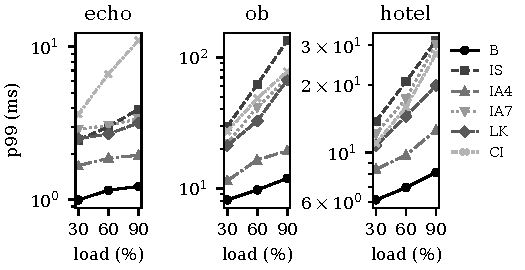
\includegraphics[width=\columnwidth]{figs/p99_carga.pdf}
  \caption{p99 latency vs.\ load level (median of 10 runs).}
  \label{fig:p99load}
\end{figure}

\begin{table*}[t]
  \centering
  \caption{p99 latency (ms), median of 10 runs. $^{*}$: different from B
           (Mann--Whitney, Holm-corrected, $p<0.05$).}
  \label{tab:p99}
  \small
  % gerado por analysis/20_estatistica.py; não editar à mão
\begin{tabular}{lrrrrrrrrr}
\toprule
Config. & echo 30\% & echo 60\% & echo 90\% & hotel 30\% & hotel 60\% & hotel 90\% & ob 30\% & ob 60\% & ob 90\% \\
\midrule
No mesh & 1.00 & 1.15 & 1.22 & 6.14 & 6.97 & 8.14 & 8.14 & 9.70 & 11.88 \\
Istio sidecar & 2.46$^{*}$ & 3.00$^{*}$ & 3.91$^{*}$ & 13.76$^{*}$ & 20.67$^{*}$ & 31.46$^{*}$ & 29.58$^{*}$ & 61.73$^{*}$ & 133.70$^{*}$ \\
Istio ambient (L4) & 1.67$^{*}$ & 1.87$^{*}$ & 1.95$^{*}$ & 8.39$^{*}$ & 9.74$^{*}$ & 12.54$^{*}$ & 11.40$^{*}$ & 16.44$^{*}$ & 19.30$^{*}$ \\
Istio ambient + waypoint & 2.88$^{*}$ & 3.07$^{*}$ & 3.38$^{*}$ & 12.11$^{*}$ & 17.35$^{*}$ & 30.35$^{*}$ & 21.95$^{*}$ & 41.51$^{*}$ & 69.31$^{*}$ \\
Linkerd & 2.51$^{*}$ & 2.69$^{*}$ & 3.17$^{*}$ & 10.73$^{*}$ & 14.49$^{*}$ & 19.88$^{*}$ & 21.10$^{*}$ & 32.56$^{*}$ & 66.88$^{*}$ \\
Cilium (WG + L7) & 3.63$^{*}$ & 6.64$^{*}$ & 10.97$^{*}$ & 10.96$^{*}$ & 15.91$^{*}$ & 27.40$^{*}$ & 27.16$^{*}$ & 48.39$^{*}$ & 77.48$^{*}$ \\
\bottomrule
\end{tabular}
% p99_ms: mediana de 10 repetições; * = diferente da B (Mann-Whitney, Holm, p<0,05)

\end{table*}

\paragraph{CPU and memory}
\Cref{fig:resources} breaks CPU down by component, normalized per
1{,}000\,req/s. At 90\% load, Ambient L4 adds the least CPU (+33\% to +61\%
depending on the application), while Cilium adds the most (+93\% on OB and
+306\% on echo). The Istio sidecar adds +215\% on echo and +116\% on HR.
The dominant component differs by design: the per-pod proxies for the Istio
sidecar and Linkerd (on OB, 4.8 and 3.6 cores per 1{,}000\,req/s), ztunnel
for Ambient L4 (2.1), ztunnel and the waypoint in similar shares for IA7 (1.3
and 1.9), and, for Cilium, the agent and the per-node Envoy in equal parts (2.6
and 3.1). Memory is mostly a fixed cost: the Istio sidecars hold 1.8\,GiB
across the 32 application pods (about 57\,MiB each), against 0.22\,GiB for
Linkerd's proxies (about 7\,MiB each); ztunnel uses about 100\,MiB in total and
the three waypoints 375\,MiB. The Istio and Linkerd control planes add about
165 and 145\,MiB on the control-plane node.

\begin{figure}[t]
  \centering
  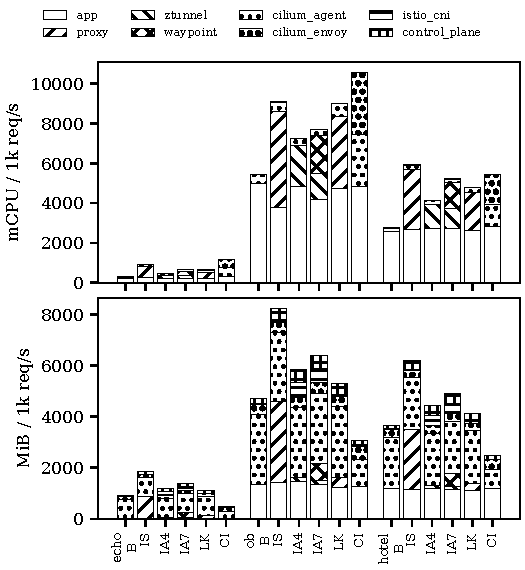
\includegraphics[width=\columnwidth]{figs/recursos.pdf}
  \caption{CPU and memory per 1{,}000\,req/s by component, at 90\% load.}
  \label{fig:resources}
\end{figure}

\paragraph{Energy}
\todo{Pending the halt-polling check. State the common idle baseline (idle
power of B), J/req per mesh, and the virtualization caveat.}

\paragraph{Variability}
Results are stable across repetitions: the coefficient of variation of p99
never exceeds 0.22 (Linkerd on OB at 90\% load). Five of the 540 runs, all on
HR, had error rates between 0.13\% and 0.38\%, and one dropped 37 requests;
all are below the 1\% threshold and are kept.

\section{RQ2: Where Does the Cost Come From?}
\label{sec:rq2}

We profiled every configuration at 60\% load on echo and OB
(\cref{sec:design}) and attribute to the data plane all samples of the proxy
processes (Envoy, \texttt{linkerd2-proxy}, ztunnel, the Cilium agent) plus any
kernel stack that runs WireGuard or an eBPF program. \Cref{fig:perfil}
breaks this CPU down per request and \cref{tab:perfil} summarizes it.

\paragraph{What each data plane spends}
On OB, the baseline spends 0.64\,ms of CPU per request in its data plane (the
Cilium CNI's eBPF programs). The Istio sidecar spends 5.5\,ms, of which 61\% is
HTTP/2 framing and header compression (\texttt{nghttp2}): with 11 internal
calls per request, each crossing two sidecars, protocol processing dominates,
as MeshInsight found for an older Envoy~\cite{zhu2023meshinsight}. Ambient L4
spends 2.6\,ms, almost half of it (47\%) in TLS inside ztunnel and no L7
parsing; adding the waypoint (IA7) raises it to 4.2\,ms, split between the
waypoint's HTTP processing (39\%) and ztunnel's TLS (31\%). Linkerd spends
4.6\,ms; because its proxy is distributed without symbols, 46\% of it can only
be attributed to the proxy as a whole, and 13\% is kernel networking. Every
mesh also multiplies kernel crossings: on OB, the proxy processes make 191
(IS) to 329 (CI) system calls and 58 to 152 context switches per request,
against 48 and 31 in the baseline.

\paragraph{Why Cilium is the slowest on echo}
On echo, Cilium spends 0.92\,ms of data-plane CPU per request, 9.6$\times$ the
baseline and 1.6$\times$ the Istio sidecar, although the request crosses a
single internal hop. Every request is redirected to the per-node Envoy by the
L7 rule on both nodes, is encrypted by WireGuard (14\% of the total), and makes
the Cilium agent spend almost as much CPU as Envoy itself (36\,s against 39\,s
over the profiling window). It also has the most context switches per request
(27, against 12 for the sidecar). We could not resolve the agent's symbols, so
we cannot say which agent function consumes this time.

\paragraph{Why the Istio sidecar is the slowest on OB}
On OB, Cilium spends even more CPU per request than the sidecar (7.2 against
5.5\,ms), yet its p99 is lower (77 against 134\,ms at 90\% load). The
difference is where the work runs. The sidecar's cost follows the frontend,
which issues all 11 internal calls through its own proxy, so it accumulates on
the frontend's node: at 90\% load that worker is 76\% utilized with the
sidecar and 68\% with Cilium, whose per-node Envoys spread L7 work over the
nodes that receive the calls. Tail latency is set by queueing on that node,
which is the mechanism behind the queueing term of our model (\cref{sec:rq3}).

\begin{figure}[t]
  \centering
  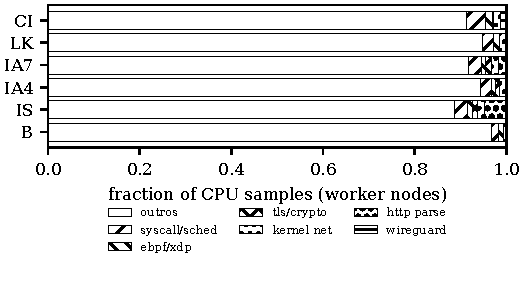
\includegraphics[width=\columnwidth]{figs/perfil.pdf}
  \caption{Data-plane CPU per request by category, at 60\% load (sum of the
           three workers).}
  \label{fig:perfil}
\end{figure}

\begin{table}[t]
  \centering
  \caption{Data-plane CPU per request at 60\% load, share spent in
           cryptography (TLS and WireGuard) and HTTP/gRPC processing, and
           context switches (cs) and system calls (sys) of the proxy
           processes per request.}
  \label{tab:perfil}
  \small
  \setlength{\tabcolsep}{3pt}
  % gerado por analysis/50_perfil.py
\begin{tabular}{llrrrrr}
\toprule
App & Config. & CPU ($\mu$s/req) & TLS+WG & HTTP & cs/req & sys/req \\
\midrule
echo & B & 95 & 0\% & 0\% & 7.6 & 12.5 \\
echo & IS & 584 & 10\% & 52\% & 12.4 & 36.8 \\
echo & IA4 & 240 & 24\% & 6\% & 12.7 & 29.9 \\
echo & IA7 & 418 & 22\% & 30\% & 15.7 & 46.9 \\
echo & LK & 389 & 0\% & 0\% & 14.0 & 30.8 \\
echo & CI & 916 & 14\% & 0\% & 26.7 & 61.7 \\
ob & B & 641 & 0\% & 0\% & 31.0 & 47.7 \\
ob & IS & 5485 & 11\% & 61\% & 58.1 & 190.6 \\
ob & IA4 & 2591 & 47\% & 10\% & 82.1 & 264.2 \\
ob & IA7 & 4206 & 31\% & 39\% & 68.9 & 302.9 \\
ob & LK & 4624 & 0\% & 0\% & 71.4 & 219.5 \\
ob & CI & 7213 & 16\% & 0\% & 151.8 & 329.2 \\
\bottomrule
\end{tabular}

\end{table}

\section{RQ3: Can the Overhead Be Predicted?}
\label{sec:rq3}

\paragraph{Model}
We model the latency added by a mesh as
\begin{equation}
  \Delta L = P_{m}(a)\, c_{m} + q_{m}\, \frac{\rho_{\text{hot}}}{1-\rho_{\text{hot}}},
  \label{eq:model}
\end{equation}
where $P_m(a)$ is the number of proxy traversals that mesh $m$ adds to a
request of application $a$, $c_m$ is the cost of one traversal,
$\rho_{\text{hot}}$ is the measured CPU utilization of the busiest worker, and
$q_m$ scales the queueing term. $P_m(a)$ comes from the call graph measured
with Istio telemetry: echo makes 1 internal call per request (across nodes),
OB 11 (10.4 across nodes), and HR 3.8 (1.0 across nodes, 2.8 on the same
node). A sidecar mesh adds two traversals per call, ztunnel one per node
crossed, and the waypoint one more per L7 call. We fit $c_m$ and $q_m$ by
non-negative least squares on echo and OB and predict HR, which is held out.

\paragraph{Results}
\Cref{tab:model} shows the prediction error. For Ambient L4 the model predicts
the p99 of HR with 11\% error (22\% for the mean), and yields a cost of
72--120\,\textmu s per ztunnel traversal. For the other meshes it does not
generalize: errors range from 82\% (Linkerd) to 140\% (Ambient with waypoint)
on p99. For the Istio sidecar and the waypoint, the fit assigns the whole
overhead to the queueing term ($c_m = 0$): on OB, the frontend and its proxy
saturate the node that hosts them, and the per-hop cost cannot be separated
from queueing on that node. We therefore read RQ3 as a partial answer. A
per-traversal model suffices when the data plane is light (L4), but for L7
data planes tail latency is governed by the utilization of the busiest node,
which depends on placement as much as on the mesh. Leaving one load level out
instead of one application gives p99 errors from 27\% (Ambient L4) to 111\%
(Istio sidecar), which confirms this reading.

\begin{table}[t]
  \centering
  \caption{Model parameters and prediction error on HR (held out). $P$:
           proxy traversals per request; $c$: fitted cost per traversal;
           LOLO: error when leaving one load level out.}
  \label{tab:model}
  \small
  \setlength{\tabcolsep}{3pt}
  % generated by analysis/41_modelo_x.py
\begin{tabular}{lrrrrrr}
\toprule
Config. & $c_p$ ($\mu$s) & $c_x$ ($\mu$s) & $q$ (ms) & err.\ HR & err.\ place. & err.\ $X_{\max}$ \\
\midrule
IS & 0 & 0 & 35.0 & 135\% & 40\% & 4\% \\
IA4 & 120 & 0 & 3.8 & 11\% & -- & 8\% \\
IA7 & 0 & 0 & 42.6 & 138\% & 27\% & 17\% \\
LK & 56 & 0 & 21.4 & 82\% & -- & 9\% \\
CI & 798 & 0 & 23.8 & 140\% & -- & 7\% \\
CI4 & 0 & 277 & 2.8 & 13\% & -- & -- \\
\bottomrule
\end{tabular}

\end{table}

\section{RQ4: Which Mesh Should I Use?}
\label{sec:rq4}

\Cref{tab:guide} condenses our results into a decision guide. Two observations
cut across it. First, the cheapest mesh is the one that does the least per
request: Ambient L4 avoids L7 parsing entirely and is the best option on every
metric we measured. Second, for L7 data planes, where the work runs matters as
much as how much work there is: shared proxies and services with a high
fan-out concentrate CPU on a few nodes, and the busiest node sets the tail, so
their placement should be part of capacity planning.

\begin{table}[t]
  \centering
  \caption{Decision guide. Evidence at 90\% load unless stated otherwise.}
  \label{tab:guide}
  \footnotesize
  \setlength{\tabcolsep}{3pt}
  \begin{tabular}{@{}p{0.27\columnwidth}p{0.17\columnwidth}p{0.5\columnwidth}@{}}
    \toprule
    Need & Choose & Evidence \\
    \midrule
    mTLS and L4 policy only & IA4 & lowest p99 increase (+54 to +62\%), 78--85\% of
      no-mesh throughput, least CPU; no L7 parsing (\cref{sec:rq2}) \\
    L7 policy, deep call graphs & LK or IA7 & p99 on OB: +463\% (LK) and +483\% (IA7)
      vs.\ +1025\% (IS) \\
    L7 on a high fan-out service & IA7, waypoint off the hot node & the sidecar
      concentrates the fan-out on one node (76\% utilized) \\
    Smallest memory footprint & IA4 or LK & ztunnel 100\,MiB in total; Linkerd
      7\,MiB per pod vs.\ 57\,MiB for Istio sidecars \\
    Already on Cilium, few L7 rules & CI, scoped L7 rules & highest data-plane CPU per
      request (0.92\,ms on echo); node Envoy, agent and WireGuard on every request \\
    \bottomrule
  \end{tabular}
\end{table}

\section{Threats to Validity}
\label{sec:threats}

\paragraph{Single host}
All VMs share one host, memory bus, and last-level cache. We mitigate this by
pinning every vCPU to a dedicated physical thread and by validating against
MeshInsight (\cref{sec:validation}), but absolute numbers will differ on
physical clusters.

\paragraph{Energy under virtualization}
RAPL measures the whole package, including the hypervisor. We found that KVM
halt-polling makes idle-heavy configurations draw more power than their
in-guest CPU use predicts.\todo{finalize after the halt-polling check}

\paragraph{Ordering}
Runs are randomized within each configuration, but configurations ran in
blocks. An interleaved control experiment (B and IS alternated in blocks)
reproduced the same power difference at the same temperatures, which rules out
time of day and temperature as its cause.

\paragraph{Versions and defaults}
Meshes evolve quickly; we pin versions and use default proxy settings, which
may not match tuned production deployments.

\paragraph{Applications}
Two benchmark applications and a microbenchmark cannot represent every call
graph; Hotel Reservation keeps most of its calls on the same node under our
placement, which favors node-level proxies.

\section{Conclusion}
\label{sec:conclusion}

We compared six service-mesh configurations on the same testbed, with open-loop
load and the same absolute request rates for all of them. Istio Ambient in L4
mode is the cheapest mesh on every metric: it keeps 78--85\% of the no-mesh
throughput and adds 54--62\% to p99 at 90\% load, while the L7 data planes add
144--1025\%. Profiling shows where the difference comes from: HTTP/2 processing for
the Istio sidecar, TLS for ztunnel, and the per-node Envoy, the agent, and
WireGuard for Cilium. Beyond per-request cost, the tail of L7 meshes is set by
the busiest node, which a per-hop model cannot capture and placement can
change. We release the testbed and data so that these results can be
reproduced and extended.


% Anonymous for review: no names, grants, or affiliations.
\section*{Acknowledgment}
The authors used Claude (Anthropic), a generative AI system in this work: to
help design the experiments, to write the testbed, measurement, and analysis
scripts, and to draft and revise the text. All experiments ran on the
authors' own hardware. The authors reviewed every script, number, and claim
against the measured data and take full responsibility for the content of
this paper.

\bibliographystyle{IEEEtran}
\bibliography{refs}

\end{document}
